%% notes-tex/026-kinetics-thermodynamics/sections/4b-coverage.tex
%% [[experiments.026-metabolism-flux.scripts.improve_parameter_coverage]]
%% https://github.com/Mjvolk3/torchcell/tree/main/notes-tex/026-kinetics-thermodynamics/sections/4b-coverage.tex

\section{Coverage, route by route\secstatus{todo}}
\label{sec:coverage}

Every number in this section is produced by a script in
\texttt{experiments/026-metabolism-flux/}, named in the source note of each figure and
table; \texttt{thermo\_pipeline\_}\allowbreak\texttt{yeast9.py},
\texttt{thermo\_curation\_}\allowbreak\texttt{price.py} and
\texttt{external\_pka\_}\allowbreak\texttt{apply\_selection.py} need the eQuilibrator env
rather than the torchcell env.

\textbf{A value with no named route is not a value.} Every one of yeast-GEM 9.0.2's 2{,}806
metabolites carries either a \emph{route}, which says how its formation energy was
produced, or an \emph{unpriced reason}, which says what stands in the way; the same holds
for each of the 4{,}131 reactions. The two partition the model exactly, and the partition
is asserted when the table is written rather than checked afterwards. This section reads
that partition out, route by route.

%% notes-tex/026-kinetics-thermodynamics/tables/thermo_vocabulary.tex
%% AUTO-GENERATED -- do not hand-edit. Regenerate with
%%   PYTHONPATH=. python experiments/026-metabolism-flux/scripts/thermo_route_tables_tex.py
%% SOURCE: hand-authored definitions declared in thermo_route_tables_tex.py, assembled from the same RouteDoc and ReasonDoc records the route tables are built from
\begin{table}[!htbp]
  \centering
  \footnotesize
  \caption[Controlled vocabulary]{Every term the recovery sections use, in alphabetical order. A route is a way of producing a value, a failure class is a reason there is none, and the two partition every species and every reaction in the model.}
  \label{tab:thermo-vocabulary}
  \begin{tabular}{@{}p{0.24\textwidth}p{0.70\textwidth}@{}}
    \toprule
    Term & Definition \\
    \midrule
    admission & the strongest claim a curation record's sources support: measured, tabulated, computed or provisional. Only measured and tabulated reach a served table \\
    cache, by accession & a route. Reads an eQuilibrator compound the model's own identifier resolves, takes its component-contribution formation energy and transforms it to the metabolite's compartment \\
    cache, by written structure & a route. Writes a structure from the metabolite's name, hashes it to an InChIKey and finds a compound eQuilibrator already holds under that key \\
    cancellation & a route. Drops a species appearing unchanged on both sides, so a reaction closes without that species ever being priced \\
    carrier potential & a route. Gauges an electron carrier pair, oxidized form at zero and reduced form at $-nFE'^{\circ}$, so the arbitrary gauge cancels in any reaction that conserves the carrier \\
    catalytic unit & one reaction and the gene product complex that catalyzes it, the key a turnover number and a Michaelis constant are stored under \\
    CODATA ion table & a route. Reads a tabulated single-ion formation energy, shifts it to eQuilibrator's gauge and applies the Debye-Huckel term \\
    component contribution & eQuilibrator's estimator: decompose a structure into groups, fit group energies against a measured reaction corpus, and return a formation energy with the covariance that fit implies \\
    composition surrogate & a route. Transfers the energy of a cache compound sharing the heavy-atom composition, admitted only where every such compound agrees to 5 kJ/mol \\
    conserved moiety & a route. Decomposes every participant leniently and prices the group difference where the atoms no group covers match as a multiset across the two sides \\
    curated structure or convention & a route. Prices a species from a structure or a polymer convention a curation record fixes, with sources and a sha256 per source \\
    decomposition refused & a failure class. the structure exists and component contribution refuses it, so a pKa predictor changes nothing \\
    evidence class & what a value rests on, one of measured, tabulated, estimated by component contribution, or curated \\
    external pKa cascade & a route. Creates a compound eQuilibrator has never seen, from the pH 7 major microspecies plus a predicted pKa ladder, then decomposes and prices it \\
    flux-carrying & a reaction whose flux-variability width is nonzero under the wild-type medium, so the layer can express a flux through it \\
    group in the null space & a failure class. the structure decomposes and one group is in the component-contribution null space, so the estimate has infinite variance \\
    microspecies & one protonation state of a compound. The reference microspecies is the state the caller draws, and choosing the neutral parent rather than the pH 7 major microspecies moves a formation energy by hundreds of kJ/mol \\
    mixed routes & a route. Sums participants priced by more than one route, so the reaction's uncertainty belongs to no single route \\
    more than one reason & a failure class. the reaction is blocked by species in two or more of the classes above \\
    no structure & a failure class. a definite formula with no structure in any namespace and no writer that composes one from the name \\
    non-chemical reaction & a failure class. an exchange, demand, sink or biomass pseudoreaction, not elementally balanced, so a standard reaction energy has no meaning for it \\
    permanently closed & a reaction no pKa predictor, structure writer, decomposer or literature table can price, because every species blocking it is not a molecule \\
    pKa ladder & the list of macroscopic dissociation constants inside pH 0 to 14 that fixes how a compound's protonation states are populated, and therefore its Legendre transform \\
    placeholder formula & a failure class. an R, X or $*$ in the formula: the species is a family of molecules and no single formation energy exists for it \\
    placeholder structure & a failure class. the only structure that resolves carries an attachment point, so the species is a residue inside a macromolecule \\
    priced & carrying a transformed formation energy at the species' own compartment conditions; a reaction is priced when every participant is, or when a reaction-level route fills it directly \\
    pseudo-metabolite & a failure class. a modeling device, a pool, a SLIME backbone or a difference formula, rather than a molecule \\
    recorded, not admitted & a failure class. a curation record exists and its admission is computed or provisional, so it is reported and not priced \\
    repeat-unit surrogate & a route. Prices one polymer residue as the monomer minus water minus half a calibrated hydrolysis energy \\
    shipped metabolite column & a route. Reads yeast-GEM's own \texttt{model\_metDeltaG.csv}, converted out of kilocalories at parse time \\
    shipped reaction column & a route. Reads yeast-GEM's \texttt{model\_rxnDeltaG.csv} directly \\
    target & one distinct structure submitted to the external pKa route. Several yeast-GEM species can share one target \\
    \bottomrule
  \end{tabular}
\end{table}


\subsection{What the tables cover\secstatus{todo}}

%% notes-tex/026-kinetics-thermodynamics/tables/thermo_coverage_ladder.tex
%% AUTO-GENERATED -- do not hand-edit. Regenerate with
%%   PYTHONPATH=. python experiments/026-metabolism-flux/scripts/thermo_route_tables_tex.py
%% SOURCE: results/parameter_coverage.json, delta_g_ladder and flux_weighted (improve_parameter_coverage.py); the last row from results/reaction_thermo_coverage_final.json (thermo_pipeline_yeast9.py)
\begin{table}[!htbp]
  \centering
  \footnotesize
  \caption[Coverage ladder]{Every source of a formation energy counted against the whole model, 4{,}131 reactions and 2{,}806 metabolites. A reaction counts only when every participant carries a value, which is the level the flux layer consumes, since the second-law hinge needs the whole stoichiometric sum; the metabolite column sits beside it because a metabolite-level figure is the one usually quoted and it overstates what is usable. The last row is the pipeline as built, which reaches every source above and eight recovery routes besides (Table~\ref{tab:thermo-metabolite-routes}). The shipped row's values are on the wrong scale, being yETFL's in kcal\,mol$^{-1}$ and labeled kilojoules (Section~\ref{sec:shipped-provenance}), so its count is a count of numbers rather than of reactions a consumer can read without a conversion.}
  \label{tab:ladder}
  \begin{tabular}{@{}lrrrrp{0.32\textwidth}@{}}
    \toprule
    Source & Rxns & \% & Mets & \% & Supplies \\
    \midrule
    yeast-GEM shipped column & 3{,}505 & 84.85 & 2{,}389 & 85.14 & kcal-scale point values, no uncertainty, this model only \\
    eQuilibrator recomputation, baseline & 2{,}741 & 66.35 & 2{,}113 & 75.30 & covariance of rank 590, any organism, any compound with a structure \\
    union of the two & 3{,}716 & 89.95 & 2{,}511 & 89.49 & covariance where the recomputation reaches, point values elsewhere \\
    union plus the tight surrogate & 3{,}730 & 90.29 & 2{,}522 & 89.88 & as the union, plus 39 species a same-composition surrogate determines \\
    union plus every surrogate & 3{,}862 & 93.49 & 2{,}574 & 91.73 & refused: the median surrogate spread is 52.6 kJ/mol, which orients nothing \\
    \midrule
    \textbf{as built} & \textbf{3{,}801} & \textbf{92.01} & \textbf{2{,}559} & \textbf{91.20} & one covariance-carrying estimate wherever one exists, and a named route and provenance record on every value \\
    \bottomrule
  \end{tabular}
  \vspace{0.3em}\\
  {\footnotesize Over the 2{,}845 reactions with nonzero flux-variability width under the wild-type medium, the last row is 2{,}724, 95.75 percent.}
\end{table}


\textbf{3{,}801 of 4{,}131 reactions carry a standard reaction energy, and 2{,}724 of the
2{,}845 that can carry flux.} Counted over chemical reactions alone, dropping the 284
exchange, demand, sink and biomass pseudoreactions for which a standard reaction energy has
no meaning, it is 3{,}535 of 3{,}847. Those three denominators answer three different
questions and none of them is the headline: the flux-carrying figure bounds what the layer
can express, the chemical figure is what a thermodynamics claim should quote, and the
whole-model figure is what a reader compares against yeast-GEM's shipped column.

\textbf{The ladder's first four rows are a comparison of sources and the last is the
pipeline.} Reading the recomputation's 66.4 percent against the shipped column's 84.9 was
never the right comparison, because the two price different reactions rather than nested
ones and only one of them carries an uncertainty. Three things separate them.

\emph{Covariance.} The recomputation returns a square-root factor of the formation-energy
error covariance, of rank 590 over 2{,}806 metabolites, so a reaction energy comes with an
uncertainty correlated with every other reaction's in the way component contribution says
it should be. The shipped file is a column of numbers with no uncertainty of any kind. Of
the reactions the built table prices, 1{,}770 carry a finite standard error, which is the
stricter figure and the one a sampler would use.

\emph{Transferability.} The shipped table was assembled by matching
yETFL~\cite{oftadehGenomescaleMetabolicModel2021} values on the metabolite name string, so
it exists for this model and no other; the recomputation works from structure and prices
all five betaxanthin intermediates (Section~\ref{sec:thermo}).

\emph{Transport terms.} \textbf{Neither table carries one, and the module now computes it},
nonzero on 326 of the 1{,}468 reactions that cross a membrane and agreeing in sign with the
GEM's own column on 84.7 percent of the 287 nonzero in both
(Section~\ref{sec:transport-term}, \texttt{results/transport\_terms.json}).
\textbf{This is the one row where the shipped table has a partial answer the recomputation
cannot reconstruct}, since yETFL's term carries a protonation contribution this module does
not.

\subsection{Every value, and the route that produced it\secstatus{todo}}
\label{sec:routes}

%% SOURCE: results/reaction_thermo_coverage_final.json and
%% results/thermo_curation_closure.json, drawn by plot_thermo_recovery_routes.py; every
%% count the panels show is written to results/thermo_recovery_routes_figure.json.
\begin{figure}[!htbp]
  \centering
  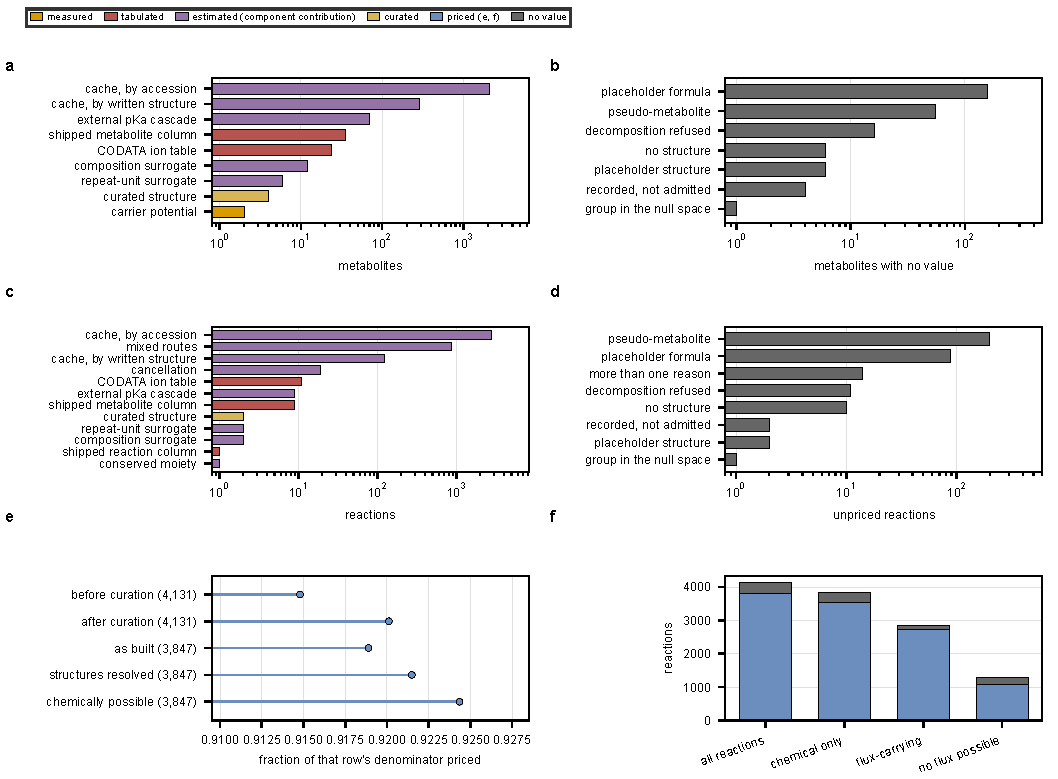
\includegraphics[width=\textwidth]{figures/thermo_recovery_routes.pdf}
  \caption[Route attribution across yeast-GEM 9.0.2]{\textbf{Which route produced each
  formation and reaction energy, and which failure class holds the rest.} Bars are colored
  by evidence class, and panels a to d use a logarithmic count axis because the routes span
  three orders of magnitude.
  \textbf{a}, The 2{,}559 priced metabolites by route. Two routes reach the eQuilibrator
  compound cache, one by an identifier the model carries and one by a structure written
  here from the metabolite's name, and together they account for 2{,}406 of them.
  \textbf{b}, The 247 metabolites with no value, by failure class. The two largest classes
  are species that are not molecules.
  \textbf{c}, The 3{,}801 priced reactions by route. \emph{Mixed routes} is a reaction whose
  participants came from more than one route, so its uncertainty belongs to no single one,
  and it is the second largest entry.
  \textbf{d}, The 330 unpriced reactions by the single failure class that blocks them,
  which partitions them exactly; \emph{more than one reason} is the class for a reaction
  blocked by species in two or more of the others.
  \textbf{e}, The ceiling ladder. Each row is a fraction of the denominator printed in its
  own tick label, because the before-and-after-curation pair exists only over the whole
  model while the three rungs are over the 3{,}847 chemical reactions; the run that
  produced the before figure did not emit a chemical denominator. Curation moved the whole
  model from 3{,}779 to 3{,}801 reactions. The last rung, 3{,}556, is what would be priced
  if every structure, ladder and refused decomposition in the model were resolved, so it is
  the ceiling for any method rather than for this one.
  \textbf{f}, Reactions priced under four denominators. The reactions no medium lets carry
  flux hold most of the remaining gap, so the flux-carrying restriction is higher than the
  whole-model figure rather than lower. Generated by
  \texttt{experiments/026-metabolism-flux/scripts/plot\_thermo\_recovery\_routes.py}.}
  \label{fig:thermo-routes}
\end{figure}

%% notes-tex/026-kinetics-thermodynamics/tables/thermo_metabolite_routes.tex
%% AUTO-GENERATED -- do not hand-edit. Regenerate with
%%   PYTHONPATH=. python experiments/026-metabolism-flux/scripts/thermo_route_tables_tex.py
%% SOURCE: results/reaction_thermo_coverage_final.json, metabolite_routes; prose column declared in thermo_route_tables_tex.py
\begin{table}[!htbp]
  \centering
  \footnotesize
  \caption[Formation-energy routes]{Every route that produced a formation energy, and how many of yeast-GEM 9.0.2's 2{,}806 metabolites it priced. The nine routes sum to the 2{,}559 priced species; the 247 with no value are Table~\ref{tab:thermo-unpriced-classes}. Evidence class is the strongest thing the number rests on, so a surrogate is estimated rather than tabulated: its value is component contribution on another molecule.}
  \label{tab:thermo-metabolite-routes}
  \begin{tabular}{@{}p{0.135\textwidth}p{0.30\textwidth}p{0.19\textwidth}lr@{}}
    \toprule
    Route & What it does & What it needs & Evidence & Species \\
    \midrule
    cache, by accession & reads an eQuilibrator compound the model's own identifier resolves, takes its component-contribution formation energy and transforms it to the metabolite's compartment & a MetaNetX, ChEBI, KEGG or BiGG identifier on the metabolite & estimated & 2{,}117 \\
    cache, by written structure & writes a structure from the metabolite's name, hashes it to an InChIKey and finds a compound eQuilibrator already holds under that key & a name stating the acyl composition, and a headgroup template & estimated & 289 \\
    external pKa cascade & creates a compound eQuilibrator has never seen, from the pH 7 major microspecies plus a predicted pKa ladder, then decomposes and prices it & a structure and a pKa ladder from the selected cascade & estimated & 70 \\
    shipped metabolite column & reads yeast-GEM's own \texttt{model\_metDeltaG.csv}, converted out of kilocalories at parse time & a row in that file for this metabolite & tabulated & 35 \\
    CODATA ion table & reads a tabulated single-ion formation energy, shifts it to eQuilibrator's gauge and applies the Debye-Huckel term & a monatomic ion whose species CODATA evaluates & tabulated & 24 \\
    composition surrogate & transfers the energy of a cache compound sharing the heavy-atom composition, admitted only where every such compound agrees to 5 kJ/mol & a definite formula the cache can decompose elsewhere & estimated & 12 \\
    repeat-unit surrogate & prices one polymer residue as the monomer minus water minus half a calibrated hydrolysis energy & a hydrolysis reaction in the model that names the monomer & estimated & 6 \\
    curated structure or convention & prices a species from a structure or a polymer convention a curation record fixes, with sources and a sha256 per source & an admitted curation record of kind structure or polymer convention & curated & 4 \\
    carrier potential & gauges an electron carrier pair, oxidized form at zero and reduced form at $-nFE'^{\circ}$, so the arbitrary gauge cancels in any reaction that conserves the carrier & a measured midpoint potential for the couple & measured & 2 \\
    \bottomrule
  \end{tabular}
\end{table}


%% notes-tex/026-kinetics-thermodynamics/tables/thermo_reaction_routes.tex
%% AUTO-GENERATED -- do not hand-edit. Regenerate with
%%   PYTHONPATH=. python experiments/026-metabolism-flux/scripts/thermo_route_tables_tex.py
%% SOURCE: results/reaction_thermo_coverage_final.json, reaction_routes; prose column declared in thermo_route_tables_tex.py
\begin{table}[!htbp]
  \centering
  \footnotesize
  \caption[Reaction-energy routes]{Every route that produced a reaction energy, over yeast-GEM 9.0.2's 4{,}131 reactions, 3{,}801 of them priced. A reaction is priced only when every participant carries a formation energy, or when a reaction-level route fills it directly, so the largest entry is the metabolite route its participants all came from and the second is the reactions assembled from more than one.}
  \label{tab:thermo-reaction-routes}
  \begin{tabular}{@{}p{0.135\textwidth}p{0.30\textwidth}p{0.19\textwidth}lr@{}}
    \toprule
    Route & What it does & What it needs & Evidence & Reactions \\
    \midrule
    cache, by accession & reads an eQuilibrator compound the model's own identifier resolves, takes its component-contribution formation energy and transforms it to the metabolite's compartment & a MetaNetX, ChEBI, KEGG or BiGG identifier on the metabolite & estimated & 2{,}751 \\
    mixed routes & sums participants priced by more than one route, so the reaction's uncertainty belongs to no single route & every participant priced by something & estimated & 872 \\
    cache, by written structure & writes a structure from the metabolite's name, hashes it to an InChIKey and finds a compound eQuilibrator already holds under that key & a name stating the acyl composition, and a headgroup template & estimated & 122 \\
    cancellation & drops a species appearing unchanged on both sides, so a reaction closes without that species ever being priced & an unpriced species identical in name, formula and charge on both sides & estimated & 19 \\
    CODATA ion table & reads a tabulated single-ion formation energy, shifts it to eQuilibrator's gauge and applies the Debye-Huckel term & a monatomic ion whose species CODATA evaluates & tabulated & 11 \\
    external pKa cascade & creates a compound eQuilibrator has never seen, from the pH 7 major microspecies plus a predicted pKa ladder, then decomposes and prices it & a structure and a pKa ladder from the selected cascade & estimated & 9 \\
    shipped metabolite column & reads yeast-GEM's own \texttt{model\_metDeltaG.csv}, converted out of kilocalories at parse time & a row in that file for this metabolite & tabulated & 9 \\
    curated structure or convention & prices a species from a structure or a polymer convention a curation record fixes, with sources and a sha256 per source & an admitted curation record of kind structure or polymer convention & curated & 2 \\
    repeat-unit surrogate & prices one polymer residue as the monomer minus water minus half a calibrated hydrolysis energy & a hydrolysis reaction in the model that names the monomer & estimated & 2 \\
    composition surrogate & transfers the energy of a cache compound sharing the heavy-atom composition, admitted only where every such compound agrees to 5 kJ/mol & a definite formula the cache can decompose elsewhere & estimated & 2 \\
    shipped reaction column & reads yeast-GEM's \texttt{model\_rxnDeltaG.csv} directly & a row in that file, with the 33 dGPredictor rows exempt from the conversion & tabulated & 1 \\
    conserved moiety & decomposes every participant leniently and prices the group difference where the atoms no group covers match as a multiset across the two sides & a curated structure for each participant and a moiety that cancels & estimated & 1 \\
    \bottomrule
  \end{tabular}
\end{table}


%% notes-tex/026-kinetics-thermodynamics/tables/thermo_route_provenance.tex
%% AUTO-GENERATED -- do not hand-edit. Regenerate with
%%   PYTHONPATH=. python experiments/026-metabolism-flux/scripts/thermo_route_tables_tex.py
%% SOURCE: prose declared in thermo_route_tables_tex.py; route list from results/reaction_thermo_coverage_final.json
\begin{table}[!htbp]
  \centering
  \footnotesize
  \caption[Route provenance]{Which committed script documents and produces each route. A route present in \file{results/thermo\_pipeline\_yeast9.json} with no entry here makes \file{thermo\_route\_tables\_tex.py} raise, so the table cannot fall behind the pipeline.}
  \label{tab:route-provenance}
  \begin{tabular}{@{}p{0.24\textwidth}p{0.66\textwidth}@{}}
    \toprule
    Route & Produced and documented by \\
    \midrule
    cache, by accession & \texttt{build\_equilibrator\_thermo.py, thermo\_accession\_sweep.py} \\
    cache, by written structure & \texttt{lipid\_structure\_writer.py} \\
    external pKa cascade & \texttt{external\_pka\_apply\_selection.py} \\
    shipped metabolite column & \texttt{yeast9\_delta\_g\_provenance.py} \\
    CODATA ion table & \texttt{fetch\_ion\_formation\_energies.py, thermo\_ion\_gauge\_check.py} \\
    composition surrogate & \texttt{improve\_parameter\_coverage.py} \\
    repeat-unit surrogate & \texttt{thermo\_polymer\_repeat\_unit.py} \\
    curated structure or convention & \texttt{thermo\_curation\_price.py, results/curation/} \\
    carrier potential & \texttt{thermo\_curation\_price.py, results/curation/cytochrome\_c.json} \\
    mixed routes & \texttt{thermo\_pipeline\_yeast9.py} \\
    cancellation & \texttt{thermo\_pipeline\_yeast9.py} \\
    shipped reaction column & \texttt{thermo\_dgpredictor\_rows.py} \\
    conserved moiety & \texttt{thermo\_curation\_price.py} \\
    \bottomrule
  \end{tabular}
\end{table}


\textbf{The cache is the workhorse and the recovery routes are the tail, and the tail is
where the errors live.} 2{,}117 metabolites come from an identifier that resolved to a
compound eQuilibrator already holds, and a further 289 from a structure written here whose
InChIKey resolved one. The remaining 153 come from seven routes each worth between 2 and 70
species, and each of those seven had to be built, checked and given a provenance record.
Their reaction yield is smaller still: 19 reactions carry the cancellation route, 9 the
external p$K_a$ cascade, 2 a curated structure and 1 a conserved moiety.
\textbf{Coverage was not what the recovery routes bought.} What they bought is a table in
which every value names its own method, so a disagreement can be attributed rather than
argued about.

\subsection{Mapping a model species onto a molecule\secstatus{todo}}
\label{sec:mapping}

Four mappings sit between the model and an estimator, and each can be silently wrong: an
identifier can resolve to the wrong compound, a name can be parsed into the wrong
structure, a polymer's residue can be counted with the wrong end groups, and a curator can
record a species the model does not actually contain.

%% SOURCE: results/thermo_pipeline_figure.json (namespaces),
%% results/thermo_curation_closure.json (composition check and curation records),
%% results/lipid_names_parsed.json, results/lipid_coverage.json,
%% results/thermo_polymer_repeat_unit.json and results/thermo_acyl_transfer.json; drawn by
%% plot_molecule_mapping.py, which writes results/molecule_mapping_figure.json.
\begin{figure}[!htbp]
  \centering
  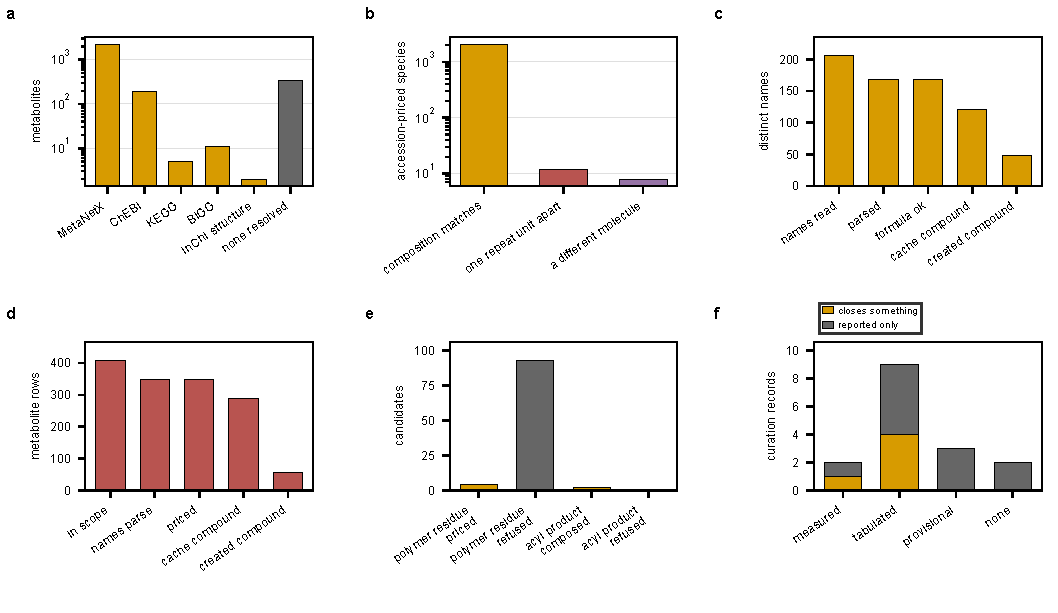
\includegraphics[width=\textwidth]{figures/molecule_mapping.pdf}
  \caption[From a model species to a molecule]{\textbf{The four mappings between a
  yeast-GEM species and a molecule an estimator can price.}
  \textbf{a}, Which namespace resolved each metabolite, in the order
  \texttt{build\_equilibrator\_thermo.py} tries them, so the bars are disjoint: a
  metabolite counted under ChEBI is one whose MetaNetX identifier missed. MetaNetX 2{,}265,
  ChEBI 191, BiGG 11, KEGG 5 and an InChI structure lookup 2, with 332 resolving nothing.
  \textbf{b}, The composition check over the 2{,}414 accession-priced species: whether the
  compound the identifier resolved carries the model's own heavy-atom composition. 2{,}087
  match, 12 are the dolichol family whose structures carry exactly one isoprene unit more
  than the model's formula, and 8 are a different molecule.
  \textbf{c}, The lipid structure writer counted in distinct names. 168 of 206 parse, all
  168 reproduce yeast-GEM's own elemental formula, 120 resolve a compound the cache already
  holds and 48 need a compound created through the external p$K_a$ route.
  \textbf{d}, The same writer counted in metabolite rows, which is the count coverage moves
  by: 347 of 409 rows priced, 289 by cache lookup and 58 through a created compound.
  \textbf{e}, The two smaller writers. The polymer repeat-unit surrogate prices 4 of 97
  candidates, refusing the rest because no hydrolysis reaction in the model identifies a
  monomer; the acyl-transfer writer composes 2 of 3 products and prices none of them,
  pricing being the p$K_a$ route's job.
  \textbf{f}, The 16 curation records by admission, split by whether the record closed a
  species or a reaction. Only \emph{measured} and \emph{tabulated} may price anything, and
  four of the nine tabulated records still close nothing because the structure they record
  is one component contribution refuses. Generated by
  \texttt{experiments/026-metabolism-flux/scripts/plot\_molecule\_mapping.py}.}
  \label{fig:molecule-mapping}
\end{figure}

\paragraph{The accession route had no composition check, and eight species were priced as a
different molecule.} It accepted the first identifier that resolved to a compound carrying
a formation energy, whatever molecule that compound is. Checking the resolved structure's
composition against yeast-GEM's own formula, over every accession-priced species, separates
three populations (Figure~\ref{fig:molecule-mapping}b). \textbf{Six prices are withdrawn and
the withdrawal costs 10 reactions}, which is the correct direction: a formation energy for
the wrong molecule is worse than none, because it produces a reaction potential with a
confident sign.

%% notes-tex/026-kinetics-thermodynamics/tables/thermo_accession_mispricings.tex
%% AUTO-GENERATED -- do not hand-edit. Regenerate with
%%   PYTHONPATH=. python experiments/026-metabolism-flux/scripts/thermo_route_tables_tex.py
%% SOURCE: results/thermo_curation_closure.json, accession_sweep.other; full per-species rows in results/thermo_accession_composition.json
\begin{table}[!htbp]
  \centering
  \footnotesize
  \caption[Accession mispricings]{The eight species the composition check found priced as a different molecule. The accession route accepted the first identifier that resolved to a compound carrying a formation energy, whatever molecule that compound is; checking the resolved structure's composition against the model's own formula over all 2{,}414 accession-priced species finds 2{,}087 matches, 12 dolichols carrying exactly one extra isoprene unit, and these eight. Six are withdrawn; the glycogen pair is re-derived per residue from a curated polymer convention instead.}
  \label{tab:thermo-mispricings}
  \begin{tabular}{@{}llllrl@{}}
    \toprule
    Species & Name & GEM formula & Priced as & $\Delta_f G'^{\circ}$ & Outcome \\
    \midrule
    \texttt{s\_0773} & glycogen & \texttt{C6H10O5} & \texttt{C24H42O21} & -1127.2 & re-derived \\
    \texttt{s\_0774} & glycogen & \texttt{C6H10O5} & \texttt{C24H42O21} & -1370.9 & re-derived \\
    \texttt{s\_1578} & zymosterol intermediate 1c & \texttt{C28H43O3} & \texttt{C29H46O2} & 1257.2 & withdrawn \\
    \texttt{s\_2920} & 3-oxo-cis-hexadec-9-enoyl-... & \texttt{C37H62N7O18P3S} & \texttt{C37H60N7O17P3S} & -575.1 & withdrawn \\
    \texttt{s\_2923} & 3-oxo-cis-octadec-9-enoyl-... & \texttt{C39H66N7O18P3S} & \texttt{C39H64N7O17P3S} & -395.1 & withdrawn \\
    \texttt{s\_4207} & trans-4-hydroxy-L-proline & \texttt{C5H9NO3} & \texttt{C5H4N4O4} & -119.0 & withdrawn \\
    \texttt{s\_4295} & dimethylallyl phosphate & \texttt{C5H9O4P} & \texttt{C8H8O} & -512.4 & withdrawn \\
    \texttt{s\_4313} & ITP & \texttt{C10H11N4O14P3} & \texttt{C4H4O4} & -2531.7 & withdrawn \\
    \bottomrule
  \end{tabular}
\end{table}


\textbf{The 12 dolichols are kept, with the offset recorded.} Every dolichol species in
yeast-GEM carries the $n = 0$ core formula while every accession structure is the $n = 1$
molecule, so the offset is one isoprene unit on both sides of any reaction that conserves
the carrier and cancels there. That is a statement about the reactions these species appear
in rather than about the values, so the offset is written into the provenance record rather
than corrected away.

\paragraph{A curation record is a claim with sources, and most of them close nothing.} Each
of the 16 records carries its own structure, potential, p$K_a$ ladder or polymer convention,
with a verbatim quote, a retrieval command and a sha256 for every source, and each records
what the group decomposer said about it. Eleven are admitted and five are not: three are
provisional, resting on another organism or on a construction rather than a measurement, and
two record that nothing was found. \textbf{An admitted record still prices nothing when the
structure it records is one component contribution refuses}, which is four of the nine
tabulated records and is the honest outcome rather than a failure of the curation.

%% notes-tex/026-kinetics-thermodynamics/tables/thermo_curation_records.tex
%% AUTO-GENERATED -- do not hand-edit. Regenerate with
%%   PYTHONPATH=. python experiments/026-metabolism-flux/scripts/thermo_route_tables_tex.py
%% SOURCE: results/thermo_curation_closure.json, rows; records in results/curation/
\begin{table}[!htbp]
  \centering
  \footnotesize
  \caption[Curation records]{The 16 hand-curated records. \emph{Admission} is the strongest claim the sources support, and only \emph{measured} and \emph{tabulated} reach the table a model reads: a provisional or absent record is loaded, validated and reported without being priced, which is why five of them price nothing. \emph{Closed} counts reactions the record itself closed, with in parentheses the reactions closed because the species cancels across the reaction instead. Each record carries its sources with a sha256 per source in \file{experiments/026-metabolism-flux/results/curation/}.}
  \label{tab:thermo-curation}
  \begin{tabular}{@{}p{0.15\textwidth}lllrrlp{0.24\textwidth}@{}}
    \toprule
    Record & Kind & Admission & Decomp. & Spec. & Src & Closed & Value \\
    \midrule
    chitobiosyl\_\-pp\_\-dolichol & polymer & tabulated & yes & 1 & 14 & 0 & repeat unit C36H64N2O17P2, no linkage stated \\
    cytochrome\_\-c & carrier & measured & n/a & 2 & 10 & 7 & E$'$0 272.0 mV vs SHE, n=1, Saccharomyces cerevi... \\
    ethylnitronate & structure & tabulated & yes & 1 & 11 & 0 & a curated structure, drawn as one microspecies \\
    glycogen & polymer & tabulated & refused & 2 & 2 & 0 & repeat unit C6H10O5, curated dGf$'$0 s\_0773 -244... \\
    heme\_\-a & structure & tabulated & refused & 3 & 7 & 1 & a curated structure, drawn as one microspecies \\
    heme\_\-o & structure & tabulated & refused & 1 & 7 & 1 & a curated structure, drawn as one microspecies \\
    mannan & polymer & tabulated & refused & 2 & 11 & 3 & repeat unit C6H10O5, curated dGf$'$0 s\_1107 -248... \\
    nitrophenyl\_\-phosphate & structure & tabulated & mixed & 2 & 7 & 0 & per metabolite: s\_3860=a structure, s\_3859=non... \\
    pectin & polymer & tabulated & refused & 1 & 18 & 0 & repeat unit C6H7O6, alpha-(1-$>$4) glycosidic, t... \\
    siroheme & structure & tabulated & refused & 1 & 11 & 0 & a curated structure, drawn as one microspecies \\
    triphosphate & pKa ladder & measured & refused & 2 & 10 & 0 (1) & pKa ladder [7.77, 5.4] \\
    cytochrome\_\-b5 & carrier & provisional & n/a & 2 & 10 & 0 & E$'$0 5.5 mV vs SHE, n=1, Bos taurus \\
    ferroheme\_\-b & pKa ladder & provisional & refused & 1 & 9 & 0 & pKa ladder [4.75, 4.15] \\
    gpi\_\-intermediate & formula & provisional & n/a & 1 & 17 & 0 & formula -$>$ C55H100N3O39P3R2 \\
    methionine\_\-s\_\-oxide & not found & none & refused & 3 & 10 & 0 & nothing found \\
    porphyrin & not found & none & refused & 2 & 9 & 0 (1) & nothing found \\
    \bottomrule
  \end{tabular}
\end{table}


\subsection{A p$K_a$ route that does not need the license\secstatus{todo}}
\label{sec:pka}

\textbf{Coverage of the native network and coverage of an inserted pathway are separate
problems.} A perturbation understood as an edit to the cell's total genomic content adds
reactions yeast-GEM never had, carrying compounds absent from the compound cache, which is
the one case the ChemAxon license governs. Adding such a compound requires the p$K_a$
constants \texttt{cxcalc} supplies, without which \texttt{LocalCompoundCache} opens
read-only; that blocker also stands behind every metabolite the structure writers reach and
the cache does not already hold.

\paragraph{The bridge is an unreleased option, and it takes p$K_a$s and nothing else.}
\texttt{equilibrator-assets} master merged \texttt{pkas\_provided\_externally} on
2026-08-15; the last PyPI release, 0.6.0 from January 2024, does not carry it, so the route
runs from a clone pinned at commit \texttt{c79e371e}. The caller passes a dictionary keyed
by the exact structure string, valued by a list of \emph{macroscopic} constants, and the
option lifts read-only mode without ChemAxon. Charge and the proton ladder are then derived
from the structure rather than supplied: the atom bag comes from the SMILES through Open
Babel, and the microspecies mapping is indexed off the hydrogen count and the number of
supplied constants above pH 7. \textbf{The reference microspecies is therefore whatever
protonation state the caller wrote the structure in, and that choice is worth
776 kJ\,mol$^{-1}$.} Pricing 7 written lipids from their neutral structures left a residual
of $-777.5$ kJ\,mol$^{-1}$ against the same compounds in the cache; submitting the pH 7
major microspecies instead leaves $+0.13$, range 0.07 to 0.15. The difference sits in two
entries of the 163-long group vector, one for the phosphate and one for the amine, so it is
the untransformed group-contribution term rather than the transform. \textbf{Submit the
pH 7 major microspecies.} The error is silent otherwise: standard InChI normalizes mobile
protons, so the two conventions share an InChIKey and a single local cache returns the
compound the first call created, which is why the comparison needs two caches that cannot
see each other.

\paragraph{The validation set is the cache's own constants, which is what makes it a test.}
No open-source predictor was trained to reproduce ChemAxon, so the cache is an independent
reference rather than a leaked one. 2{,}400 compounds are drawn from the 694{,}324 the cache
holds, stratified on constant count, functional group, mass and whether the compound is
lipid-like, and the 2{,}100 outside the pinned seed-17 300 are what every number below is
measured on. The pinned 300 are excluded because ensemble membership was fitted on them.

\paragraph{The rule is a tail bound at every compartment pH, not an average error.} A method
is scored by the \emph{worst} per-pH 90th percentile of
$|\Delta_f G'^{\circ}(\textrm{predicted}) - \Delta_f G'^{\circ}(\textrm{cache})|$ over the
eight pHs the pipeline transforms at, subject to a failure rate of at most 0.02, breaking
ties on the pH 7.2 median and then on cost. Three choices in that sentence are doing work.
The p90 rather than the mean, because the fill-in is a tail risk and one wrongly signed
reaction potential is what a second-law hinge acts on. The worst pH rather than the mean
over pHs, because a metabolite is priced at its own compartment's pH and a good cytosol
score would otherwise hide a bad vacuole one. And a failure-rate bound rather than a scored
error, because a method that cannot answer leaves a gap rather than a cheap answer.

%% notes-tex/026-kinetics-thermodynamics/tables/pka_method_selection.tex
%% AUTO-GENERATED -- do not hand-edit. Regenerate with
%%   PYTHONPATH=. python experiments/026-metabolism-flux/scripts/pka_selection_table_tex.py
%% SOURCE: results/pka_method_selection.json, rule and ranking, written by external_pka_method_selection.py decide
\begin{table}[!htbp]
  \centering
  \footnotesize
  \caption[pKa method selection]{Every candidate p$K_a$ method against the eQuilibrator compound cache's own ChemAxon constants, on the 2{,}100 held-out compounds. The rule selects the smallest \emph{worst} per-pH p90 of $|\Delta\Delta_f G'^{\circ}|$ among methods whose failure rate is at most 0.02, breaking ties on the pH 7.2 median and then on cost. Failure rate is the fraction of compounds a method returns no ladder for, and it is a bound rather than a scored error because a method that cannot answer leaves a gap rather than a cheap answer. \emph{Right count} is the fraction whose ladder length matches the cache's, reported and deliberately outside the rule: a ladder can carry the right number of constants and the wrong values, and the transform is what the flux layer consumes.}
  \label{tab:pka-selection}
  \begin{tabular}{@{}llrrrrrrl@{}}
    \toprule
    & & & \multicolumn{2}{c}{worst pH} & \multicolumn{2}{c}{at pH 7.2} & & \\
    Method & Kind & Fail & p90 & pH & Median & Mean & Right count & Verdict \\
    \midrule
    median of two & ensemble & 0.1695 & 7.83 & 5 & 0.502 & 1.47 & 0.282 & rejected, failure rate 0.170 \\
    cascade, three members & ensemble & 0.0024 & 8.33 & 7.8 & 0.067 & 1.04 & 0.338 & \textbf{selected} \\
    cascade, two members & ensemble & 0.0029 & 8.33 & 7.8 & 0.068 & 1.04 & 0.338 & ranked below \\
    Uni-pKa, simple template & tool & 0.1152 & 8.75 & 7.8 & 0.077 & 1.16 & 0.354 & rejected, failure rate 0.115 \\
    best tool per functional group & ensemble & 0.1152 & 8.75 & 7.8 & 0.077 & 1.16 & 0.354 & rejected, failure rate 0.115 \\
    MolGpKa & tool & 0.0571 & 9.33 & 7.8 & 0.130 & 1.10 & 0.217 & rejected, failure rate 0.057 \\
    median of three & ensemble & 0.0048 & 9.38 & 7.8 & 0.331 & 1.80 & 0.364 & ranked below \\
    pKasolver-lite & tool & 0.0071 & 18.12 & 7.8 & 1.466 & 4.05 & 0.364 & ranked below \\
    \bottomrule
  \end{tabular}
  \vspace{0.3em}\\
  {\footnotesize p90, median and mean are of $|\Delta\Delta_f G'^{\circ}|$ in kJ\,mol$^{-1}$.}
\end{table}


%% notes-tex/026-kinetics-thermodynamics/tables/pka_p90_by_ph.tex
%% AUTO-GENERATED -- do not hand-edit. Regenerate with
%%   PYTHONPATH=. python experiments/026-metabolism-flux/scripts/pka_selection_table_tex.py
%% SOURCE: results/pka_method_selection_figure.json, panel b, written by plot_pka_method_selection.py
\begin{table}[!htbp]
  \centering
  \footnotesize
  \caption[pKa error by compartment pH]{The p90 of $|\Delta\Delta_f G'^{\circ}|$, in kJ\,mol$^{-1}$, at each pH the pipeline transforms a metabolite at. A metabolite is priced at its own compartment's pH, so a method has to hold at all eight; scoring at pH 7.2 alone understates the selected cascade's tail by 3.4 kJ\,mol$^{-1}$ and ranks MolGpKa above Uni-pKa. The mitochondrial matrix at pH 7.8 is the worst column for every method but one.}
  \label{tab:pka-by-ph}
  \begin{tabular}{@{}lrrrrrrrr@{}}
    \toprule
    & \multicolumn{8}{c}{compartment pH} \\
    Method & 5 & 6.2 & 6.6 & 7 & 7.1 & 7.2 & 7.4 & 7.8 \\
    \midrule
    median of two & 7.83 & 2.19 & 2.17 & 3.50 & 4.01 & 4.48 & 5.46 & 7.76 \\
    \textbf{cascade, three members} & 5.58 & 1.88 & 2.50 & 3.94 & 4.38 & 4.88 & 5.98 & 8.33 \\
    cascade, two members & 5.58 & 1.89 & 2.50 & 3.95 & 4.39 & 4.89 & 5.98 & 8.33 \\
    Uni-pKa, simple template & 5.56 & 1.94 & 2.75 & 4.39 & 4.89 & 5.41 & 6.48 & 8.75 \\
    best tool per functional group & 5.56 & 1.94 & 2.75 & 4.39 & 4.89 & 5.41 & 6.48 & 8.75 \\
    MolGpKa & 8.46 & 2.39 & 2.83 & 3.36 & 3.56 & 4.00 & 5.38 & 9.33 \\
    median of three & 9.34 & 2.66 & 2.65 & 4.06 & 4.60 & 5.25 & 6.46 & 9.38 \\
    pKasolver-lite & 12.58 & 3.87 & 3.88 & 7.02 & 8.28 & 9.63 & 12.27 & 18.12 \\
    \bottomrule
  \end{tabular}
\end{table}


\textbf{No single tool is admissible except the worst one.} Uni-pKa on the simple
enumeration template carries the smallest error of any single tool and returns no ladder for
11.5 percent of the compounds; MolGpKa fails on 5.7 percent, and 126 of its 2{,}400 empty
ladders come back with no error at all, 93 of them lipid-like. Only pKasolver-lite clears
the failure bound alone, at more than twice everyone else's error. \textbf{So the selected
method is a cascade rather than a tool}: Uni-pKa's answer where it has one, MolGpKa's where
it does not, pKasolver-lite's where neither does. Composition rather than averaging, because
a median is undefined at a rank where the best member returned nothing.

\textbf{The choice between the three-member and the two-member cascade is a tie the rule
breaks arbitrarily}, 8.331 against 8.333 kJ\,mol$^{-1}$, a difference of 0.02 percent. The
rule picks the three-member cascade because it is deterministic; the two-member one is the
defensible cheaper choice and nothing measured here separates them.

%% SOURCE: results/external_pka_applied.json, results/pka_method_selection.json and
%% results/pka_method_selection_figure.json, drawn by plot_pka_outside_equilibrator.py,
%% which writes results/pka_outside_equilibrator_figure.json.
\begin{figure}[!htbp]
  \centering
  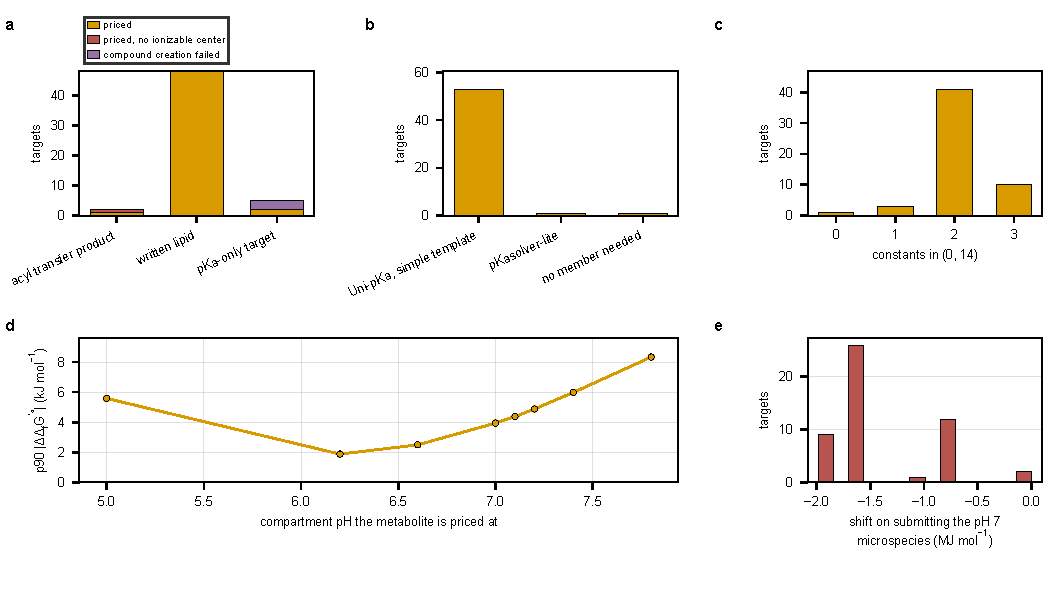
\includegraphics[width=\textwidth]{figures/pka_outside_equilibrator.pdf}
  \caption[The external pKa route on yeast-GEM]{\textbf{What the selected cascade was asked
  to do on yeast-GEM 9.0.2, and how large the two shifts a ladder controls are.} A target is
  one distinct structure; several model species can share one, and the 52 targets that yield
  a value carry the 70 metabolite rows the route table counts, 68 of them from a target with
  an ionizable center.
  \textbf{a}, The 55 targets by where they came from, partitioned by outcome. 48 are lipids
  the structure writer composed and the cache does not hold, 5 are species needing only a
  ladder, and 2 are acyl-transfer products. Three fail at compound creation and one is
  created as a single microspecies because a SMARTS scan finds no ionizable center in it,
  which is the correct answer rather than an error.
  \textbf{b}, Which cascade member answered. Uni-pKa on the simple template served 53 and
  pKasolver-lite 1, so the cascade degenerates to its first member on this population and
  earns its place on the benchmark rather than here.
  \textbf{c}, Ladder length, the number of constants inside pH 0 to 14 the cascade returned.
  Two is the mode, as expected for a phosphodiester lipid headgroup.
  \textbf{d}, The Legendre-transform error a ladder carries, as the p90 of
  $|\Delta\Delta_f G'^{\circ}|$ at each of the eight working compartment pHs over the
  2{,}100 held-out benchmark compounds. The mitochondrial matrix at pH 7.8 is the worst
  column, 8.33 kJ\,mol$^{-1}$, against 4.88 at pH 7.2, which is why the rule reads the worst
  pH rather than the cytosolic one.
  \textbf{e}, The reference-microspecies shift, which is three orders of magnitude larger
  than the ladder error: the signed change in each target's transformed formation energy
  when the pH 7 major microspecies replaces the neutral parent the writer emitted, median
  $-1{,}585$ kJ\,mol$^{-1}$ over the 50 targets priced both ways. Generated by
  \texttt{experiments/026-metabolism-flux/scripts/plot\_pka\_outside\_equilibrator.py}.}
  \label{fig:pka-outside}
\end{figure}

\textbf{An earlier 300-compound benchmark at pH 7.2 alone ranks the tools the same way and
carries three breakdowns the 2{,}400-compound run does not repeat}, per functional group,
per ladder length, and each tool's shift against each other tool's
(Table~\ref{tab:external-pka}, Figure~\ref{fig:external-pka}). Two of its findings are load
bearing. The enumeration template rather than the network decides Uni-pKa's answer: the same
weights and the same code on the full template give 2.94 kJ\,mol$^{-1}$ against the simple
template's 0.91, because the enumerator walks outward from the neutral parent and the rungs
it adds are near pH 7 by construction, which is where the transform is most sensitive. And
the tools do not agree with each other: MolGpKa against pKasolver-lite gives $r = 0.085$,
with a median absolute difference between two tools' shifts larger than the best tool's own
median error against the cache.

%% notes-tex/026-kinetics-thermodynamics/tables/external_pka_tools.tex
%% AUTO-GENERATED -- do not hand-edit. Regenerate with
%%   python experiments/026-metabolism-flux/scripts/external_pka_table_tex.py
%% SOURCE: experiments/026-metabolism-flux/results/external_pka_benchmark.json,
%% read through `external_pka_benchmark.py table`.
\begin{table}[H]
  \centering
  \footnotesize
  \caption[External pKa predictors]{Open-source p$K_a$ predictors against the compound cache's own ChemAxon-derived constants, over 300 sampled compounds at pH 7.2, I = 0.25 M, T = 303.15 K, pMg 3. The last three columns are the change in $\Delta_f G'^{\circ}$ when the predicted constants replace the cache's, with the reference microspecies and the untransformed formation energy held fixed, so they isolate the p$K_a$ contribution. \textbf{The two Uni-pKa rows are the same weights and the same code}, and differ only in the microstate enumeration template, which fixes how many rungs a ladder can have before the network is consulted. \textbf{QupKake is unmeasured on this set}: a rung costs a full xTB wave, the run reached 4 of up to 14 rungs, and only 1 of 60 ladders had terminated. Its truncated row scores all 60 with the rungs that ran, so those numbers bound it rather than measure it.}
  \label{tab:external-pka}
  \begin{tabular}{@{}lrrrrrrr@{}}
    \hline
    \multicolumn{5}{@{}l}{} & \multicolumn{3}{c@{}}{$\Delta_f G'^{\circ}$ error (kJ\,mol$^{-1}$)} \\
    Tool & $n$ & Scored & Right count & p$K_a$ MAE & MAE & Median & p90 \\
    \hline
    pKasolver-lite & 300 & 298 & 0.356 & 2.59 & 2.52 & 0.56 & 6.40 \\
    MolGpKa & 300 & 294 & 0.248 & 2.83 & 1.21 & 0.34 & 3.20 \\
    Uni-pKa, full template & 300 & 300 & 0.200 & 2.54 & 2.94 & 1.11 & 7.93 \\
    Uni-pKa, simple template & 300 & 299 & 0.324 & 2.79 & 0.91 & 0.16 & 2.84 \\
    QupKake & 60 & 1 & 0.000 & 4.56 & 1.87 & 1.87 & 1.87 \\
    QupKake, truncated & 60 & 60 & 0.283 & 3.61 & 1.35 & 0.38 & 5.08 \\
    \hline
  \end{tabular}
\end{table}


%% SOURCE: results/external_pka_per_compound.csv, with every number the panels show
%% written to results/external_pka_figure.json; figure by plot_external_pka.py.
\begin{figure}[!htbp]
  \centering
  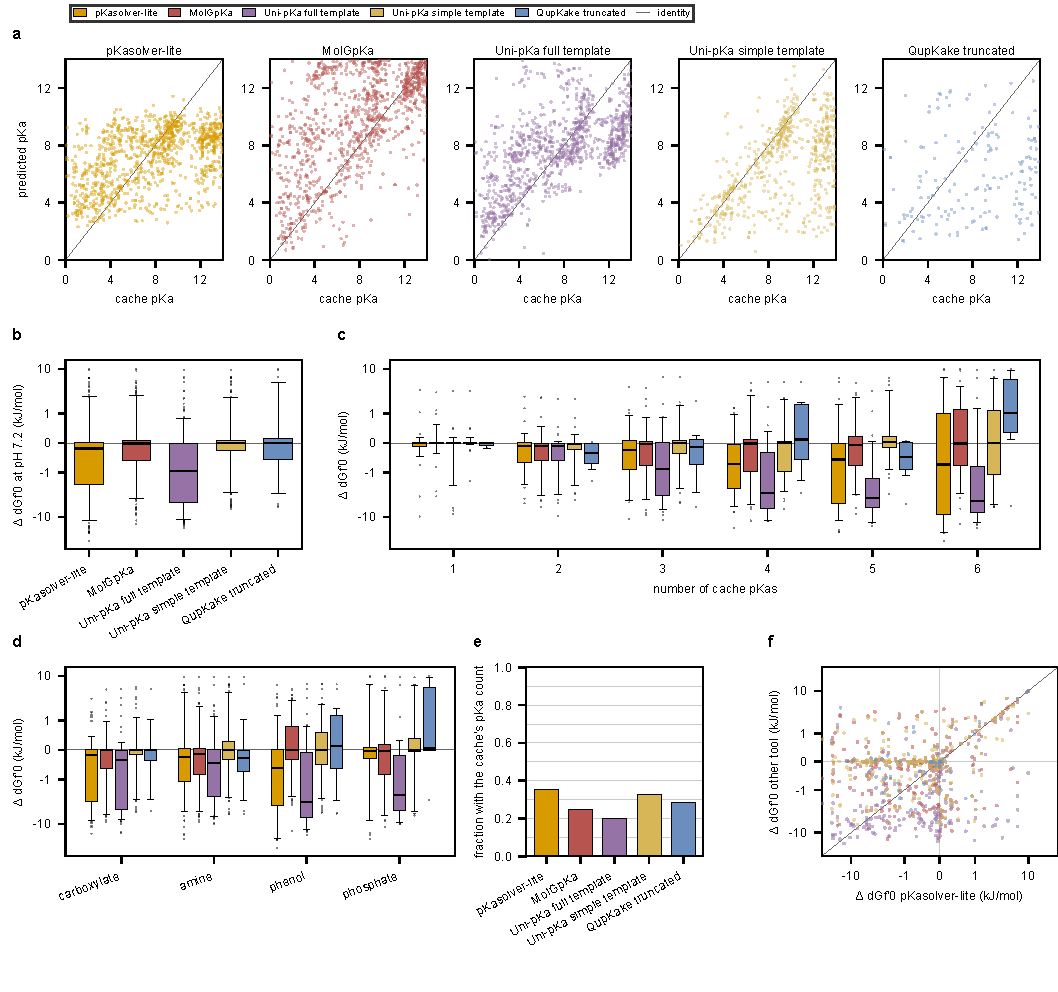
\includegraphics[width=\textwidth]{figures/external_pka_benchmark.pdf}
  \caption[Open-source pKa predictors against the cache]{\textbf{Four open-source p$K_a$
  predictors against the compound cache's ChemAxon constants, on 300 compounds at pH 7.2.}
  This is the earlier and smaller benchmark; the selection of Table~\ref{tab:pka-selection}
  runs on 2{,}100 held-out compounds at eight pHs and supersedes its ranking.
  \textbf{a}, Predicted against cache p$K_a$, paired by rank over the shorter of the two
  lists, on 1{,}010 pairs for pKasolver-lite, 1{,}021 for MolGpKa, 1{,}043 for the full
  template, 596 for the simple template and 167 for truncated QupKake; the simple template is
  the only cloud that follows the identity line, with 0.374 of its pairs inside 1 p$K_a$ unit
  against MolGpKa's 0.358, the full template's 0.267 and pKasolver-lite's 0.258, on half as
  many pairs.
  \textbf{b}, Signed change in $\Delta_f G'^{\circ}$ per compound; every median sits just
  below zero, so what separates the tools is tail width, at 5th percentiles of $-12.19$
  kJ\,mol$^{-1}$ for pKasolver-lite, $-11.22$ for the full template, $-3.93$ for MolGpKa and
  $-2.87$ for the simple template.
  \textbf{c}, The same shift split by the number of constants the cache holds, where the full
  template's error grows monotonically from 0.64 to 5.43 kJ\,mol$^{-1}$ across the six strata
  while the simple template's spans 0.14 to 2.13.
  \textbf{d}, The same shift split by functional group; the simple template is the smallest
  in all four, 1.03 against MolGpKa's 1.35 on amine, 0.71 against 1.00 on carboxylate, 1.08
  against 1.18 on phenol and 1.75 against 2.33 on phosphate.
  \textbf{e}, Fraction of compounds whose constant count matches the cache's, 0.356
  pKasolver-lite, 0.324 simple template, 0.248 MolGpKa, 0.200 full template, which ranks the
  tools differently from the energy columns.
  \textbf{f}, Each tool's per-compound shift against pKasolver-lite's, which is the question
  of whether the predictors agree with one another: they do not, at $r = 0.085$ for MolGpKa
  and 0.268 for the simple template, with median absolute differences of 0.74 and 0.62
  kJ\,mol$^{-1}$, larger than the simple template's own median error against the cache.
  QupKake is drawn only as its truncated row. Generated by
  \texttt{experiments/026-metabolism-flux/scripts/plot\_external\_pka.py}.}
  \label{fig:external-pka}
\end{figure}

\textbf{A ladder that is wrong is worth about ten kilojoules, and a reference microspecies
that is wrong is worth about eight hundred.} Those two are the whole error budget of this
route, and they are not comparable in size. The ladder error is measured against the cache's
own constants and runs to a p90 of 8.33 kJ\,mol$^{-1}$ at the worst compartment pH; the
reference-microspecies error is a fixed offset in the group-contribution term and moved the
48 written lipids by a median of 1{,}585 kJ\,mol$^{-1}$ when it was corrected. A worked case
of the first is triphosphate: the cache stores a six-microspecies ladder one rung too far in
both directions, and against the measured ladder the two Legendre transforms differ by
\textbf{12.762 kJ\,mol$^{-1}$}. That is what the cached ladder would inject into
\texttt{r\_4403} the day an anchor for triphosphate exists, so the measured ladder is
recorded now and prices nothing on its own.

\textbf{Magnesium is the gap this route cannot close.} \texttt{specified\_pkas} carries
proton dissociation constants only, and \texttt{Compound.transform} reads magnesium through
the microspecies table that is materialized once at creation, so a constant appended
afterwards commits and changes nothing. Omitting them costs 0.0018 to 4.12 kJ\,mol$^{-1}$ at
pMg 3 on the benchmark compounds that carry any, always in the direction of
under-stabilizing the compound, and up to 9.43 at pMg 2. Carrying a constant over by
substructure is worse than omitting it: bucketing eQuilibrator's own 535-compound table by
ionizable phosphate steps leaves a within-bucket standard deviation of 1.6 to 3.3 log units,
and a p$K_d$ off by 2 costs 10.87 kJ\,mol$^{-1}$ on 5-formyl-THF and 11.14 on ADP against
4.12 and 1.10 for having no constant at all.

One interface defect belongs with these. The guard tests truthiness rather than presence, so
an empty list, the correct answer for a compound with no constant between pH 0 and 14, raises
rather than creating a single-microspecies compound. Downstream the route tests for an
ionizable center by SMARTS instead of reading a tool's error string, because the three
cascade members word ``nothing here'' three different ways and one of them words it as an
error.

\subsection{Writing the missing lipid structures\secstatus{todo}}
\label{sec:lipids}

The 409 metabolite rows with a definite formula and no structure in any namespace are lipids
whose acyl composition is written into the name, so the structure is derivable from the name
even though no database indexes it. \texttt{lipid\_structure\_writer.py} parses each name
into a headgroup template and a list of acyl chains, assembles the SMILES in RDKit, and
prices the result two ways.

\textbf{168 of the 206 distinct names parse, covering 347 of the 409 metabolite rows, and
all 168 reproduce yeast-GEM's own elemental formula exactly.} The 38 that do not split into
17 SLIME backbone pseudo-metabolites, whose formula is a difference formula rather than a
molecule, and 21 names with no acyl composition to read: glycans, hemes, cytochromes,
protein-linked lysines and a GPI anchor. Every double bond is placed at $\Delta$-9 and cis,
a convention yeast-GEM's \texttt{16:1} does not state; the written free acids hash to the
InChIKeys of palmitoleic and oleic acid, which is what the build asserts rather than the
convention.

\textbf{All 168 price, 120 by finding a compound eQuilibrator already holds and 48 through
the external p$K_a$ route.} The cache lookup is a route the coverage audit had no structure
to key on, and it checks the structures independently: 120 written InChIKeys resolve a
compound nobody here drew.

\textbf{What this buys is method consistency rather than coverage.} The eQuilibrator route
moves from 66.35 to 86.27 percent of reactions, passing the shipped column's 84.85, and
every one of those values now comes from one group-contribution method with an uncertainty
attached. \textbf{The union with the shipped table does not move at all}, staying at 3{,}716
reactions, because that table already prices these lipids by name out of yETFL and
ModelSEED.

%% SOURCE: results/lipid_names_parsed.json, results/lipid_structures.json,
%% results/lipid_priced.json (dgf_route_difference_same_protonation_kj_per_mol) and
%% results/lipid_coverage.json, all written by lipid_structure_writer.py; figure by
%% plot_lipid_structures.py.
\begin{figure}[!htbp]
  \centering
  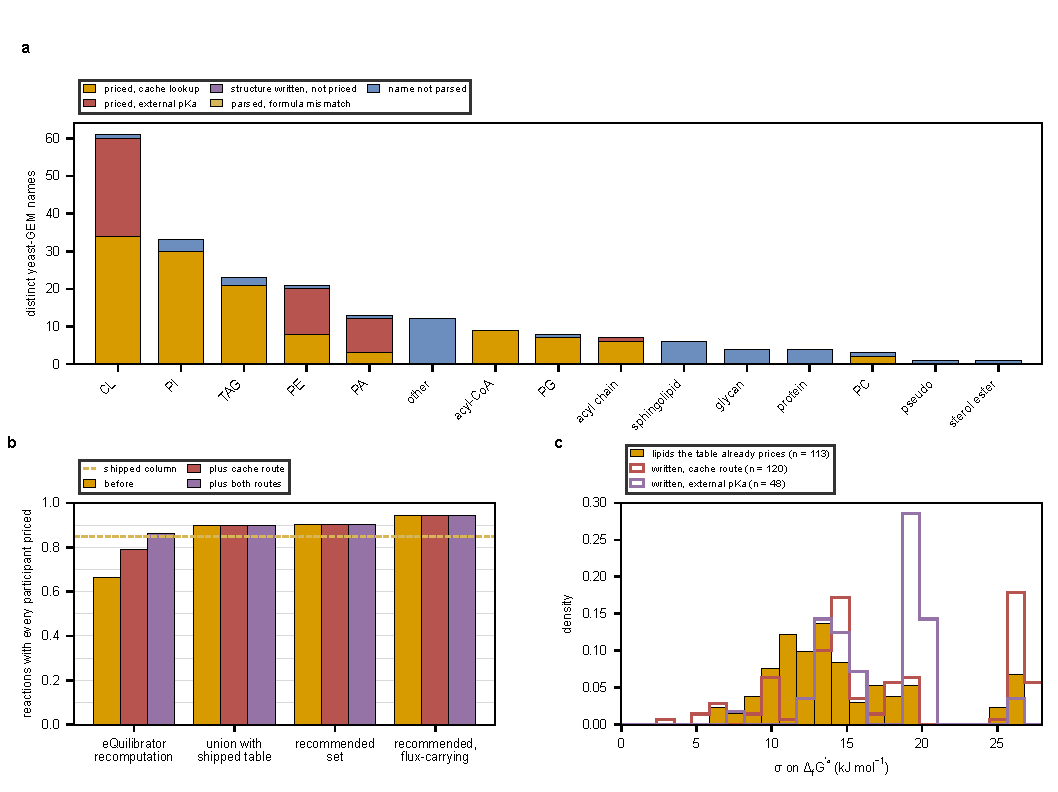
\includegraphics[width=\textwidth]{figures/lipid_structure_writer.pdf}
  \caption[The lipid structure writer: reach, coverage and uncertainty]{\textbf{What the
  lipid structure writer reached, and what it bought.}
  \textbf{a}, The 206 distinct names by yeast-GEM chemical class, each bar partitioned into
  the five mutually exclusive stages of the pipeline. No name is lost to a formula mismatch
  and none to a written structure that failed to price, so those two segments are empty
  everywhere; the whole loss is the 38 names the parser refuses.
  \textbf{b}, Reactions of 4{,}131 with every participant priced, at four levels of
  aggregation, before the written lipids, with the 120 names that resolve an existing cache
  compound, and with all 168. Dashed, the shipped metabolite column's 84.85 percent. The
  eQuilibrator recomputation crosses it; the union with the shipped table and the
  flux-carrying restriction do not move.
  \textbf{c}, Uncertainty on the formation energy, one value per distinct name: the 113
  lipid names the recomputed table already prices, the 120 written names priced by cache
  lookup, and the 48 priced through a created compound. Medians 13.19, 14.79 and
  18.92\,kJ\,mol$^{-1}$, so a written structure is priced no less certainly than a lipid the
  table already held. Generated by
  \texttt{experiments/026-metabolism-flux/scripts/plot\_lipid\_structures.py}.}
  \label{fig:lipid-writer}
\end{figure}

\subsection{Composition matching cannot buy coverage\secstatus{todo}}

455 unpriced metabolites have a heavy-atom composition that the compound cache can already
decompose, which invites pricing them from a same-composition surrogate. The test is to
price every cache compound of the same composition and measure how far apart they land.

\textbf{They land far apart.} Across the 441 metabolites that gain a value, the median
spread within a composition is \textbf{52.6\,kJ/mol} and the 90th percentile is
342\,kJ/mol. Only \textbf{39} fall below 5\,kJ/mol. At 303\,K, $RT\ln 10$ is 5.8\,kJ/mol,
so the median surrogate is uncertain by roughly nine orders of magnitude in the equilibrium
constant, which is not a constraint on a sign. Wiring all 441 in would report coverage of
93.49 percent, three and a half points above the union, on values that cannot orient a
reaction. The 39 tight ones are offered and 12 are taken by the built table, the rest
refused: \textbf{a resolution rate and a usable rate are different quantities}, and only the
second constrains a model. The 5\,kJ/mol admission bound is a judgment rather than a
measured threshold, $RT\ln 10$ rounded down.

\subsection{What is left, and which of it is permanent\secstatus{todo}}
\label{sec:permanent}

%% notes-tex/026-kinetics-thermodynamics/tables/thermo_unpriced_classes.tex
%% AUTO-GENERATED -- do not hand-edit. Regenerate with
%%   PYTHONPATH=. python experiments/026-metabolism-flux/scripts/thermo_route_tables_tex.py
%% SOURCE: results/reaction_thermo_coverage_final.json (metabolite_reasons, reactions_by_sole_blocking_reason, ceiling_ladder.permanently_closed_reasons) and results/thermo_exclusions.json (reactions_blocked_by_reason)
\begin{table}[!htbp]
  \centering
  \footnotesize
  \caption[Failure classes]{Every class that holds a value back, the species it holds and the reactions it blocks. \emph{Species} counts metabolites carrying that reason; \emph{blocks} counts reactions with at least one such participant, so the column double counts a reaction blocked by two classes; \emph{sole} counts reactions this class alone blocks and partitions the 330 unpriced reactions exactly. A class marked permanent is one no pKa predictor, structure writer, decomposer or literature table can move, so the sum of the permanent rows is the ceiling for any method rather than for this one.}
  \label{tab:thermo-unpriced-classes}
  \begin{tabular}{@{}p{0.16\textwidth}p{0.34\textwidth}p{0.17\textwidth}rrr@{}}
    \toprule
    Class & What it means & What it would take & Species & Blocks & Sole \\
    \midrule
    pseudo-metabolite$^{\dagger}$ & a modeling device, a pool, a SLIME backbone or a difference formula, rather than a molecule & none; the ceiling & 55 & 213 & 201 \\
    placeholder formula$^{\dagger}$ & an R, X or $*$ in the formula: the species is a family of molecules and no single formation energy exists for it & none; the ceiling & 159 & 99 & 89 \\
    decomposition refused & the structure exists and component contribution refuses it, so a pKa predictor changes nothing & a decomposition, or a tabulated value & 16 & 13 & 11 \\
    no structure & a definite formula with no structure in any namespace and no writer that composes one from the name & a structure from a namespace or a curator & 6 & 10 & 10 \\
    more than one reason & the reaction is blocked by species in two or more of the classes above & every blocking class resolved & 0 & 0 & 14 \\
    placeholder structure$^{\dagger}$ & the only structure that resolves carries an attachment point, so the species is a residue inside a macromolecule & none; the ceiling & 6 & 3 & 2 \\
    recorded, not admitted & a curation record exists and its admission is computed or provisional, so it is reported and not priced & a measured or tabulated source & 4 & 5 & 2 \\
    group in the null space & the structure decomposes and one group is in the component-contribution null space, so the estimate has infinite variance & a measurement of a compound carrying that group & 1 & 1 & 1 \\
    non-chemical reaction$^{\dagger}$ & an exchange, demand, sink or biomass pseudoreaction, not elementally balanced, so a standard reaction energy has no meaning for it & none; excluded from the chemical denominator & 0 & 0 & 0 \\
    \bottomrule
  \end{tabular}
  \vspace{0.3em}\\
  {\footnotesize $^{\dagger}$ permanent under the admission rule.}
\end{table}


\textbf{291 of the 330 unpriced reactions are closed for good.} A reaction is permanently
closed when every metabolite blocking it is not a molecule: a placeholder formula naming a
family, a SLIME backbone whose formula is a difference formula, or a residue inside a
macromolecule. No p$K_a$ predictor, structure writer, decomposer or literature table changes
any of those. The 21 that remain are what the last two rungs of
Figure~\ref{fig:thermo-routes}e would close, and the probe that measured them found none of
the refused structures reachable by the reactant-contribution path or by a surrogate inside
the admitted spread, so that rung needs new data rather than new code.

\textbf{Five chemistries are permanently refused for a reason that is about eQuilibrator's
group system rather than about the species.} The porphyrin macrocycle has no group, so heme
a, heme o, siroheme and ferroheme b decompose nowhere and are closable only at the reaction
level where the macrocycle cancels. The sulfoxide of L-methionine S-oxide has no group.
4-nitrophenyl phosphate, an aryl phosphate, has none either. The nitro group is the opposite
case and is worth separating: the group \emph{exists} and sits in the component-contribution
null space, carried by 0 of 631 training compounds, so the estimate has infinite variance
rather than no value. Triphosphate is a fourth kind again: it decomposes nowhere and appears
in none of the 3{,}999 training reactions, so the reactant-contribution path that prices
phosphate and diphosphate despite their empty group vectors is closed to it too. Placeholder
and R-group species are the fifth, and are a property of the model.

\paragraph{Five defects in yeast-GEM 9.0.2 were found while curating, and they are upstream
rather than ours.} Heme a's declared charge of $-3$ is chemically unreachable: no
microspecies of \texttt{C49H55FeN4O6} carries it, the ferrous dianion being
\texttt{C49H54FeN4O6} at $-2$, so every curated structure fails a strict charge comparison
against the model. \texttt{r\_0530}'s stoichiometry disagrees with EC 1.17.99.9, which
matters beside the $-440.539$ kJ\,mol$^{-1}$ the conserved-moiety route prices it at. Pectin
\texttt{s\_1309} is written at charge 0 and the galacturonate residue is $-1$, which is why
that reaction fails a charge balance. \texttt{s\_3934}, named ``Ethylnitronate'', is
nitroethane: the reaction it appears in balances only with \texttt{C2H5NO2} at charge 0, and
the nitronate anion leaves it short one hydrogen and one negative charge. And
\texttt{s\_0332}'s GPI formula was invented by a solver in 2018 rather than derived, which
is why walking the pathway from the last intermediate that carries a formula gives a
different one. The dolichol convention above is a sixth, and unlike these five it is
internally consistent and merely undocumented.

\subsection{The kinetic tables, tier by tier\secstatus{todo}}
\label{sec:kinetic-tiers}

%% notes-tex/026-kinetics-thermodynamics/tables/kinetic_tiers.tex
%% AUTO-GENERATED -- do not hand-edit. Regenerate with
%%   PYTHONPATH=. python experiments/026-metabolism-flux/scripts/kinetic_tier_tables_tex.py
%% SOURCE: results/kinetic_coverage_closure.json, parameters.k_cat.variants.verified_substrate_key_with_homolog.tier_counts; tier definitions declared in kinetic_tier_tables_tex.py
\begin{table}[!htbp]
  \centering
  \footnotesize
  \caption[Kinetic tiers]{The four tiers a turnover number or Michaelis constant is drawn from, tried in this order over the 3{,}728 catalytic units of yeast-GEM 9.0.2. $k_{cat}$ and $K_M$ resolve on the same keys and land on the same counts, because a unit that has one measured has the other. The homolog tier is measured and is nonetheless folded in with the predictions wherever an experimental fraction is reported, since a measurement of another organism's enzyme is not a measurement of this one.}
  \label{tab:kinetic-tiers}
  \begin{tabular}{@{}p{0.18\textwidth}p{0.27\textwidth}p{0.28\textwidth}rr@{}}
    \toprule
    Tier & Keyed on & Evidence about & Units & Share \\
    \midrule
    measured, this organism & the unit's own UniProt accession in the Open Enzyme Database mirror, and the assay substrate matched by InChIKey connectivity block to a substrate the reaction consumes & this protein doing this chemistry & 97 & 2.6\% \\
    measured, same EC, another organism & an EC number annotated on the reaction plus the same substrate match, in any organism & the chemistry, not this protein, so it is never counted as a measurement of the modeled organism & 782 & 21.0\% \\
    predicted & the protein sequence and the substrate structure & the median over the predictors the within-class study admits, which is EZKinetics, EITLEM and UniKP for $k_{cat}$ and EZKinetics alone for $K_M$ & 2{,}831 & 75.9\% \\
    organism default & nothing; it is the fallback & the median of the values the database tiers placed in this same table, so it is a summary of the organism rather than of the unit & 18 & 0.5\% \\
    \bottomrule
  \end{tabular}
\end{table}


%% SOURCE: results/kinetic_coverage_closure.json and
%% results/parameter_coverage_selected.json, with the Wilson intervals read from
%% results/within_class_plausibility.json; drawn by plot_kinetics_tiers.py, which writes
%% results/kinetics_tiers_figure.json.
\begin{figure}[!htbp]
  \centering
  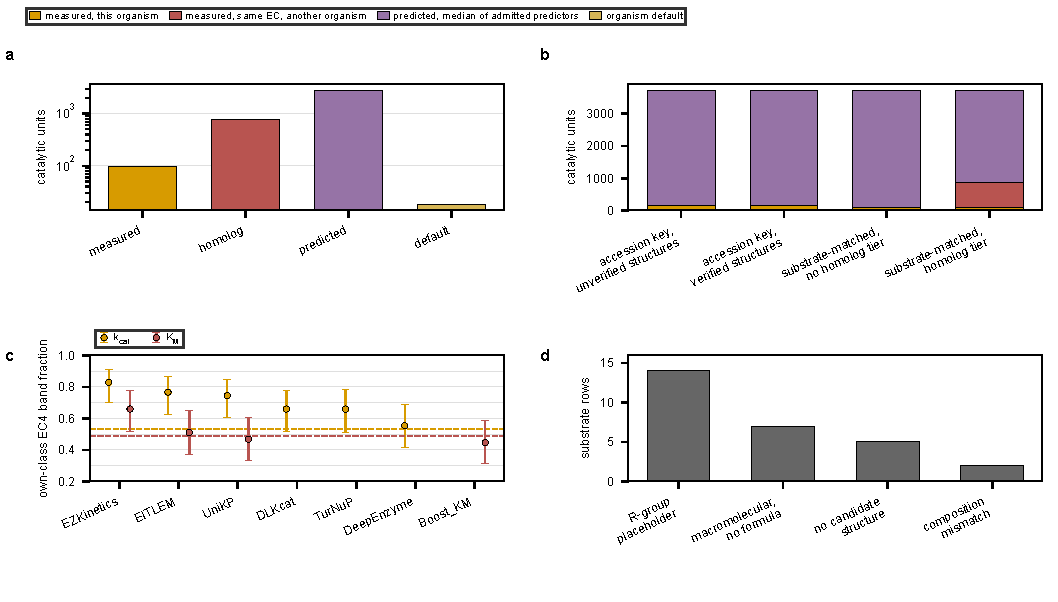
\includegraphics[width=\textwidth]{figures/kinetics_tiers.pdf}
  \caption[Kinetic tiers and the admission rule]{\textbf{What the resolved $k_{cat}$ and
  $K_M$ tables are made of, and the rule that decides which predictors may fill them.}
  \textbf{a}, The four tiers over the 3{,}728 catalytic units, on a logarithmic count axis.
  97 units carry a measurement of the modeled organism's own protein on a substrate the
  reaction consumes, 782 a measurement of the same chemistry in another organism, 2{,}831 a
  predictor median and 18 the organism default.
  \textbf{b}, The same counts under each table version. Keying the measured tier on a
  substrate match rather than on the accession alone takes it from 148 units to 97, which is
  a correction rather than a loss: 51 of the 148 accession matches were assaying a substrate
  the reaction does not consume. Verifying every substrate structure moved 8 units onto the
  default. The homolog tier recovers 33 of those 51, whose chemistry is measured elsewhere,
  and 18 fall to a predictor.
  \textbf{c}, The admission rule. Each point is a predictor's fraction of measured pairs
  landing inside the band of enzymes sharing its own EC4 class, with the study's Wilson 95
  percent interval; the dashed line is the EC-median lookup's point fraction for that
  parameter. A predictor is admitted only when its lower bound clears the line, which keeps
  EZKinetics, EITLEM and UniKP for $k_{cat}$ and EZKinetics and CatPred for $K_M$. EITLEM's
  $K_M$ lower bound is 0.383 against the lookup's 0.500, so it is refused on the parameter
  it is admitted on for turnover, and CatPred is refused on turnover while clearing the bar
  on affinity, the mirror of the same split.
  \textbf{d}, The 28 substrate rows behind the 18 units still on the default, by why no
  open-source tool reaches them. Generated by
  \texttt{experiments/026-metabolism-flux/scripts/plot\_kinetics\_tiers.py}.}
  \label{fig:kinetics-tiers}
\end{figure}

\textbf{Two and a half percent of the model's turnover numbers are measurements of its own
enzymes, and a further 21 percent are measurements of the same chemistry somewhere else.}
The homolog tier is the largest single change of this round and it is deliberately not
counted as experimental: a cross-organism EC match is a real measurement of a real enzyme,
and not of the enzyme in this model. Where both are available it is also the better
estimate, closer to the measured value than the predictor median on 55 of the 87 units
carrying both, at a median absolute error of 0.094 decades against 0.300.

%% notes-tex/026-kinetics-thermodynamics/tables/kinetic_default_units.tex
%% AUTO-GENERATED -- do not hand-edit. Regenerate with
%%   PYTHONPATH=. python experiments/026-metabolism-flux/scripts/kinetic_tier_tables_tex.py
%% SOURCE: results/kinetic_coverage_closure.json, ceiling.remaining, written by improve_kinetic_coverage.py
\begin{table}[!htbp]
  \centering
  \footnotesize
  \caption[Units on the organism default]{Every catalytic unit still carrying the organism default, and the substrate that keeps it there. A unit needs a structure for at least one substrate its reaction consumes; these have none any mirrored predictor can take. \emph{Rows} is how many of the unit's substrates fail. None of the four classes is reachable with an open-source tool: an R-group placeholder is a curation decision in the model rather than a missing structure, a macromolecular substrate needs a predictor that accepts a protein and all seven mirrored models take a small-molecule SMILES, and the structure writer was run on the last two classes and refused them.}
  \label{tab:kinetic-defaults}
  \begin{tabular}{@{}rllp{0.30\textwidth}p{0.22\textwidth}r@{}}
    \toprule
    Unit & Reaction & Genes & Substrate & Why & Rows \\
    \midrule
    556 & \texttt{r\_0520} & YKL165C & 6-O-[alpha-D-mannosyl-(1-\textgreater{}4)-alpha-D-g; phosphatidylethanolamine backbone & macromolecular species with no formula in the GEM & 2 \\
    559 & \texttt{r\_0523} & YDR302W & 6-O-\{alpha-D-mannosyl-(1-\textgreater{}2)-alpha-D-m; phosphatidylethanolamine backbone & macromolecular species with no formula in the GEM & 2 \\
    560 & \texttt{r\_0523} & YLL031C & 6-O-\{alpha-D-mannosyl-(1-\textgreater{}2)-alpha-D-m; phosphatidylethanolamine backbone & macromolecular species with no formula in the GEM & 2 \\
    1379 & \texttt{r\_1228} & YBR180W & N,N'-diformyldityrosine & no candidate structure in any mirrored catalog for this ... & 1 \\
    1565 & \texttt{r\_2148} & YHR067W & 3-hydroxybutanoyl-ACP & R-group placeholder, the GEM defines the species only up... & 1 \\
    1566 & \texttt{r\_2149} & YHR067W & 3-hydroxyhexanoyl-ACP & R-group placeholder, the GEM defines the species only up... & 1 \\
    1567 & \texttt{r\_2150} & YHR067W & 3-hydroxyoctanoyl-ACP & R-group placeholder, the GEM defines the species only up... & 1 \\
    3277 & \texttt{r\_4152} & YAL039C & Cytochrome c & candidate structures exist but none matches the GEM's co... & 1 \\
    3278 & \texttt{r\_4152} & YKL087C & Cytochrome c & candidate structures exist but none matches the GEM's co... & 1 \\
    3414 & \texttt{r\_4239} & YGL017W & Arg-tRNA(Arg); generic protein & R-group placeholder, the GEM defines the species only up... & 2 \\
    3458 & \texttt{r\_4277} & YLR099C & 1-acyl-sn-glycerol 3-phosphate; Acyl-CoA & R-group placeholder, the GEM defines the species only up... & 2 \\
    3459 & \texttt{r\_4277} & YPR139C & 1-acyl-sn-glycerol 3-phosphate; Acyl-CoA & R-group placeholder, the GEM defines the species only up... & 2 \\
    3462 & \texttt{r\_4280} & YLR239C & Apoprotein; octanoyl-ACP & R-group placeholder, the GEM defines the species only up... & 2 \\
    3463 & \texttt{r\_4281} & YLR239C & Apoprotein; Lipoyl-[acp] & R-group placeholder, the GEM defines the species only up... & 2 \\
    3505 & \texttt{r\_4325} & YOR226C & S-sulfanyl-[L-cysteine desulfurase]; [disordered-form [Fe-S] cluster scaffo & macromolecular species with no formula in the GEM & 2 \\
    3506 & \texttt{r\_4325} & YPL135W & S-sulfanyl-[L-cysteine desulfurase]; [disordered-form [Fe-S] cluster scaffo & macromolecular species with no formula in the GEM & 2 \\
    3662 & \texttt{r\_4700} & YIL166C & hydrogen sulfide & no candidate structure in any mirrored catalog for this ... & 1 \\
    3665 & \texttt{r\_4704} & YIL166C & alkanesulfonate & R-group placeholder, the GEM defines the species only up... & 1 \\
    \bottomrule
  \end{tabular}
\end{table}


\textbf{Eighteen units reach the organism default and none of them is reachable with an
open-source tool.} Fourteen of the 28 substrate rows behind them carry an R-group
placeholder, which is a curation decision in the model rather than a missing structure;
seven are macromolecular species with no formula, which need a predictor that accepts a
protein substrate and all eight mirrored models take a small-molecule SMILES; five have no
candidate structure in any mirrored catalog and the substrate writer was run on them and
refused each one; two are cytochrome c, where the model writes only the heme part of a
protein-bound species. \textbf{A substrate the writer tried and refused counts as
unreachable whatever its reason class}, which is what makes this a ceiling rather than a
backlog.

\subsection{The kinetic ceiling is substrate structure, not the models\secstatus{todo}}

DLKcat, UniKP, EITLEM and EZKinetics cover exactly the same 3{,}552 of 3{,}728 catalytic
units on the unverified tables, and DeepEnzyme covers 3{,}546. Four independently trained
models agreeing to the unit is not a coincidence about the models: every gene has a
sequence, so the binding constraint is whether the substrate has a structure to featurize.
\textbf{The 95.3 percent ceiling is a property of the inputs, and no better predictor moves
it.} Two structure routes moved it instead. Resolving an outdated MetaNetX cross-reference
priced 27 substrates, and supplying the lipid writer's own structures priced 48 more,
between them closing 165 of the 176 units that had no prediction at all. TurNuP's 55.2
percent is a model limitation rather than an input one (Section~\ref{sec:accuracy}).

The consensus tables take the per-unit median across the admitted predictors in log space
and carry the across-predictor spread beside it. \textbf{For $k_{cat}$ that spread has a
median of 0.74 orders of magnitude over the three admitted predictors and the 3{,}709 units
all three price}, down from 1.14 across all predictors, and 30.1 percent of units still
disagree by more than a factor of ten. It is concentrated rather than uniform: units whose
substrate has fewer than 12 heavy atoms sit at 0.55 decades and those above 60 heavy atoms
at 1.38, and two-gene units at 1.20 against 0.71 for single-gene ones. A $k_{cat}$ consensus
at 0.74 is still a factor of five, so the table is an order-of-magnitude prior rather than a
measurement. \textbf{For $K_M$ the admitted set became two when CatPred was scored, so a
spread exists there for the first time}, and it is narrow: a median of 0.30 orders of
magnitude over 3{,}701 units with 8.6 percent past a factor of ten. Two models agreeing is
not two models being right, and the within-class study remains the honest uncertainty.
%% SOURCE: results/kinetic_predictor_spread_with_catpred.json (overall,
%% by_substrate_heavy_atoms, by_complex_size), written by kinetic_predictor_spread.py
%% --suffix _with_catpred; the 1.14 across all predictors is
%% results/parameter_coverage_selected_with_catpred.json, k_cat.all_predictors.

%% SOURCE: results/parameter_coverage.json (panels a-f) and
%% results/parameter_coverage_selected_with_catpred.json (panels e, g, h: the rule, the
%% per-predictor statistic, and both spread distributions), both written by
%% plot_parameter_coverage.py; the plausibility fractions come from
%% results/within_class_plausibility.json.
\begin{figure}[!htbp]
  \centering
  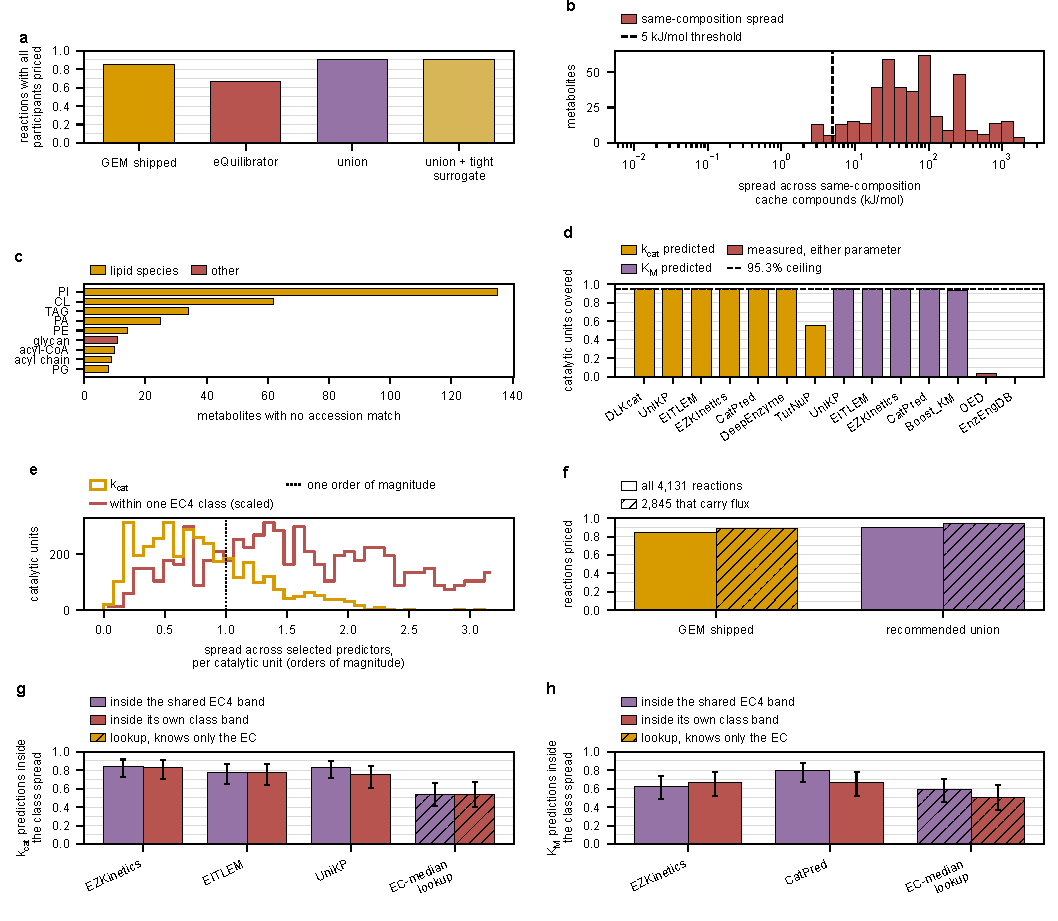
\includegraphics[width=\textwidth]{figures/parameter_coverage.pdf}
  \caption[Parameter coverage across yeast-GEM 9.0.2]{\textbf{Coverage of the three
  parameter tables across yeast-GEM 9.0.2, and what coverage means.}
  \textbf{a}, Reactions with every participant priced, by source. The union of the shipped
  table and the eQuilibrator recomputation exceeds either alone by 211 reactions, because
  the two price different reactions rather than nested ones.
  \textbf{b}, Spread of formation energy across cache compounds sharing a metabolite's
  heavy-atom composition. The dashed line is the 5\,kJ/mol threshold below which a
  composition is taken to determine the energy; 39 of 441 clear it, so composition matching
  is rejected as a coverage route.
  \textbf{c}, Metabolites with no accession match, by chemical class; orange is a lipid
  species and red is anything else. The gap is lipids: phosphatidylinositol, cardiolipin
  and triacylglycerol species alone account for 231 of 332.
  \textbf{d}, Per-predictor coverage of the 3{,}728 catalytic units. Six of the seven
  $k_{cat}$ predictors and four of the five $K_M$ predictors sit at the same
  95.1 to 95.3 percent ceiling, which is set by substrate structure availability rather than by any
  model. TurNuP's 55.2 percent is its own limitation. The two red bars are what measured
  sources supply on the accession key alone, before the substrate match of
  Section~\ref{sec:kinetic-tiers} corrects them: the Open Enzyme Database prices 138 units,
  3.7 percent, and EnzEngDB prices none, since it holds no $k_{cat}$ or $K_M$ field and no
  \emph{S. cerevisiae} content (Section~\ref{sec:accuracy}).
  \textbf{e}, Across-predictor spread per catalytic unit, over the \emph{admitted}
  predictors of panels g and h. Restricting to three of the seven $k_{cat}$ predictors takes
  the median spread from 1.14 to \textbf{0.72 orders of magnitude} and the fraction of units
  disagreeing by more than a factor of ten from 61.8 to 29.3 percent. The red outline is the
  spread across the distinct enzymes of one EC4 class, rescaled since it counts 523 classes
  rather than 3{,}698 units, so its shape and not its height is the comparison. \textbf{Even
  after selection the $k_{cat}$ spread sits inside the biological one rather than below it.}
  \textbf{f}, The same coverage counted over all reactions and over only the 2{,}845 that
  can carry flux at nonzero FVA width. Restricting to reactions the medium permits raises
  the recommended union from 90.3 to 94.4 percent.
  \textbf{g}, Within-class plausibility for the admitted $k_{cat}$ predictors, against the
  EC-median lookup drawn hatched. The rule reads the Wilson lower bound against the lookup's
  point fraction of 0.542: EZKinetics 0.704, EITLEM 0.635 and UniKP 0.612 clear it, and
  CatPred 0.525, DLKcat 0.517, TurNuP 0.511 and DeepEnzyme 0.412 do not. Accuracy on the
  measured pairs is deliberately not in the rule, since a recalled value lands inside a
  class band no more readily than a correct one, and CatPred is the case that makes the
  distinction concrete: 51 of its 58 $k_{cat}$ pairs are in its own training table
  (Section~\ref{sec:catpred}).
  \textbf{h}, The same for $K_M$, where the rule now keeps \textbf{two}: EZKinetics and
  CatPred both clear the lookup's 0.500 at a lower bound of 0.525, and EITLEM 0.383,
  UniKP 0.345 and Boost\_KM 0.314 do not. A predictor a table lookup beats is not evidence
  about the enzyme.}
  \label{fig:coverage}
\end{figure}

\subsection{Changelog\secstatus{todo}}

\textbf{2026-09-11.} Coverage closed. Formation energies: 3{,}801 of 4{,}131 reactions
priced, 3{,}535 of the 3{,}847 chemical ones and 2{,}724 of the 2{,}845 that can carry flux,
each value carrying one of nine routes and each gap one of seven failure classes. Eight
accession prices were found to be for a different molecule, six of them withdrawn. Sixteen
curation records landed, eleven admitted. Kinetics: 97 measured, 782 homolog, 2{,}831
predicted and 18 default over 3{,}728 catalytic units, on tables whose every substrate
structure passes a composition check. This section was rewritten around the route
attribution; the earlier version reported the recomputation at 66.4 percent, which is now
the baseline row of Table~\ref{tab:ladder} rather than the result.

\textbf{2026-09-12.} CatPred added as the eighth mirrored predictor and folded into every
predictor comparison in this document: the distribution, agreement, plausibility, EC-class,
coverage and tier figures all now carry eight series, and the accuracy, status and
within-class tables eight rows. It is refused for $k_{cat}$ by one hit at 32 of 48 and
admitted for $K_M$, which gives that parameter two admitted predictors and a spread for the
first time. \texttt{predictor\_vs\_measured} and \texttt{ec\_class\_variance} were
regenerated at the same time and recovered one measured pair each of the five predictors
that had been extended to the appended coverage rows, so their scorable set moved from 57
to 58 and the own-class denominator from 47 to 48.
